% Options for packages loaded elsewhere
\PassOptionsToPackage{unicode}{hyperref}
\PassOptionsToPackage{hyphens}{url}
%
\documentclass[
]{article}
\usepackage{lmodern}
\usepackage{amssymb,amsmath}
\usepackage{ifxetex,ifluatex}
\ifnum 0\ifxetex 1\fi\ifluatex 1\fi=0 % if pdftex
  \usepackage[T1]{fontenc}
  \usepackage[utf8]{inputenc}
  \usepackage{textcomp} % provide euro and other symbols
\else % if luatex or xetex
  \usepackage{unicode-math}
  \defaultfontfeatures{Scale=MatchLowercase}
  \defaultfontfeatures[\rmfamily]{Ligatures=TeX,Scale=1}
\fi
% Use upquote if available, for straight quotes in verbatim environments
\IfFileExists{upquote.sty}{\usepackage{upquote}}{}
\IfFileExists{microtype.sty}{% use microtype if available
  \usepackage[]{microtype}
  \UseMicrotypeSet[protrusion]{basicmath} % disable protrusion for tt fonts
}{}
\makeatletter
\@ifundefined{KOMAClassName}{% if non-KOMA class
  \IfFileExists{parskip.sty}{%
    \usepackage{parskip}
  }{% else
    \setlength{\parindent}{0pt}
    \setlength{\parskip}{6pt plus 2pt minus 1pt}}
}{% if KOMA class
  \KOMAoptions{parskip=half}}
\makeatother
\usepackage{xcolor}
\IfFileExists{xurl.sty}{\usepackage{xurl}}{} % add URL line breaks if available
\IfFileExists{bookmark.sty}{\usepackage{bookmark}}{\usepackage{hyperref}}
\hypersetup{
  pdftitle={Computer Assignment 2 - Exploratory Analysis},
  pdfauthor={Rui Li},
  hidelinks,
  pdfcreator={LaTeX via pandoc}}
\urlstyle{same} % disable monospaced font for URLs
\usepackage[margin=1in]{geometry}
\usepackage{color}
\usepackage{fancyvrb}
\newcommand{\VerbBar}{|}
\newcommand{\VERB}{\Verb[commandchars=\\\{\}]}
\DefineVerbatimEnvironment{Highlighting}{Verbatim}{commandchars=\\\{\}}
% Add ',fontsize=\small' for more characters per line
\usepackage{framed}
\definecolor{shadecolor}{RGB}{248,248,248}
\newenvironment{Shaded}{\begin{snugshade}}{\end{snugshade}}
\newcommand{\AlertTok}[1]{\textcolor[rgb]{0.94,0.16,0.16}{#1}}
\newcommand{\AnnotationTok}[1]{\textcolor[rgb]{0.56,0.35,0.01}{\textbf{\textit{#1}}}}
\newcommand{\AttributeTok}[1]{\textcolor[rgb]{0.77,0.63,0.00}{#1}}
\newcommand{\BaseNTok}[1]{\textcolor[rgb]{0.00,0.00,0.81}{#1}}
\newcommand{\BuiltInTok}[1]{#1}
\newcommand{\CharTok}[1]{\textcolor[rgb]{0.31,0.60,0.02}{#1}}
\newcommand{\CommentTok}[1]{\textcolor[rgb]{0.56,0.35,0.01}{\textit{#1}}}
\newcommand{\CommentVarTok}[1]{\textcolor[rgb]{0.56,0.35,0.01}{\textbf{\textit{#1}}}}
\newcommand{\ConstantTok}[1]{\textcolor[rgb]{0.00,0.00,0.00}{#1}}
\newcommand{\ControlFlowTok}[1]{\textcolor[rgb]{0.13,0.29,0.53}{\textbf{#1}}}
\newcommand{\DataTypeTok}[1]{\textcolor[rgb]{0.13,0.29,0.53}{#1}}
\newcommand{\DecValTok}[1]{\textcolor[rgb]{0.00,0.00,0.81}{#1}}
\newcommand{\DocumentationTok}[1]{\textcolor[rgb]{0.56,0.35,0.01}{\textbf{\textit{#1}}}}
\newcommand{\ErrorTok}[1]{\textcolor[rgb]{0.64,0.00,0.00}{\textbf{#1}}}
\newcommand{\ExtensionTok}[1]{#1}
\newcommand{\FloatTok}[1]{\textcolor[rgb]{0.00,0.00,0.81}{#1}}
\newcommand{\FunctionTok}[1]{\textcolor[rgb]{0.00,0.00,0.00}{#1}}
\newcommand{\ImportTok}[1]{#1}
\newcommand{\InformationTok}[1]{\textcolor[rgb]{0.56,0.35,0.01}{\textbf{\textit{#1}}}}
\newcommand{\KeywordTok}[1]{\textcolor[rgb]{0.13,0.29,0.53}{\textbf{#1}}}
\newcommand{\NormalTok}[1]{#1}
\newcommand{\OperatorTok}[1]{\textcolor[rgb]{0.81,0.36,0.00}{\textbf{#1}}}
\newcommand{\OtherTok}[1]{\textcolor[rgb]{0.56,0.35,0.01}{#1}}
\newcommand{\PreprocessorTok}[1]{\textcolor[rgb]{0.56,0.35,0.01}{\textit{#1}}}
\newcommand{\RegionMarkerTok}[1]{#1}
\newcommand{\SpecialCharTok}[1]{\textcolor[rgb]{0.00,0.00,0.00}{#1}}
\newcommand{\SpecialStringTok}[1]{\textcolor[rgb]{0.31,0.60,0.02}{#1}}
\newcommand{\StringTok}[1]{\textcolor[rgb]{0.31,0.60,0.02}{#1}}
\newcommand{\VariableTok}[1]{\textcolor[rgb]{0.00,0.00,0.00}{#1}}
\newcommand{\VerbatimStringTok}[1]{\textcolor[rgb]{0.31,0.60,0.02}{#1}}
\newcommand{\WarningTok}[1]{\textcolor[rgb]{0.56,0.35,0.01}{\textbf{\textit{#1}}}}
\usepackage{graphicx,grffile}
\makeatletter
\def\maxwidth{\ifdim\Gin@nat@width>\linewidth\linewidth\else\Gin@nat@width\fi}
\def\maxheight{\ifdim\Gin@nat@height>\textheight\textheight\else\Gin@nat@height\fi}
\makeatother
% Scale images if necessary, so that they will not overflow the page
% margins by default, and it is still possible to overwrite the defaults
% using explicit options in \includegraphics[width, height, ...]{}
\setkeys{Gin}{width=\maxwidth,height=\maxheight,keepaspectratio}
% Set default figure placement to htbp
\makeatletter
\def\fps@figure{htbp}
\makeatother
\setlength{\emergencystretch}{3em} % prevent overfull lines
\providecommand{\tightlist}{%
  \setlength{\itemsep}{0pt}\setlength{\parskip}{0pt}}
\setcounter{secnumdepth}{-\maxdimen} % remove section numbering
\usepackage{amsgen,amsmath,amstext,amsbsy,amsopn,amssymb,mathabx,amsthm,bm,bbm}
\usepackage[labelsep=space]{caption}

\title{Computer Assignment 2 - Exploratory Analysis}
\usepackage{etoolbox}
\makeatletter
\providecommand{\subtitle}[1]{% add subtitle to \maketitle
  \apptocmd{\@title}{\par {\large #1 \par}}{}{}
}
\makeatother
\subtitle{\(\textbf{Machine Learning, Spring 2020}\)}
\author{Rui Li}
\date{}

\begin{document}
\maketitle

The purpose of this assignment is to walk you through a typical starting
analysis of real-world data in \texttt{R}. We will also introduce how to
draw from various probability distributions using built-in \texttt{R}
functions.

\hypertarget{inputoutput}{%
\subsection{Input/Output}\label{inputoutput}}

\texttt{scan} and \texttt{read.table} are the two main functions in
\texttt{R} for reading data. The main difference between them lies in
that \texttt{scan} reads one component (also called ``field'') at a time
while \texttt{read.table} reads one line at a time. Thus,
\texttt{read.table} requires the data to have a table structure and will
create a data.frame in \textbf{R} automatically, while \texttt{scan} can
be flexible but might require effort in manipulating data after reading.
Overall, their usages are quite similar. One should pay attention to the
frequently used options \texttt{file}, \texttt{header}, \texttt{sep},
\texttt{dec}, \texttt{skip}, \texttt{nmax}, \texttt{nlines} and
\texttt{nrows} in their \textbf{R} documents.

\texttt{write.table} is the converse of \texttt{read.table}. While the
latter reads data into \texttt{R} from a file, the former writes data to
a file from \texttt{R}.

\emph{Note:} If, in the future, you have data stored in another format,
\emph{e.g.} EXCEL or SAS dataset, then you can output it as a CSV file
and read it into \textbf{R} via the \texttt{read.csv} function (which is
almost identical to \texttt{read.table}).

\hypertarget{questions}{%
\subsubsection{Questions}\label{questions}}

In the folder for HW 1, you can find data on the 1974 Motor Trend US
Magazine on a series of road tests they did.

\begin{enumerate}
\def\labelenumi{\arabic{enumi}.}
\tightlist
\item
  Read the data using read.csv into a data frame called
  \texttt{mtcars\_dat}. This dataset is actually available in base
  \texttt{R}, but for practice use the read.csv() function.
\end{enumerate}

\begin{quote}
Important: When reading files into R that are in local directories,
you'll need to set your working directory to the place where the file is
located. Do this by going
\texttt{Session-\textgreater{}Set\ Working\ Directory-\textgreater{}Choose\ Directory...}
and choosing the file in which the data is located.
\end{quote}

\begin{quote}
Important as well: You have just been given the specific functions you
will need to solve this exercise. Don't know how to use them? Google
them! Or check the manual page for them by inputting
\texttt{?read.table()}! Coding in general requires this sort of
independence and tenacity.
\end{quote}

\begin{Shaded}
\begin{Highlighting}[]
\NormalTok{mtcars_dat =}\StringTok{ }\KeywordTok{read.csv}\NormalTok{(}\StringTok{"mtcars.csv"}\NormalTok{)}
\end{Highlighting}
\end{Shaded}

Use \texttt{str(mtcars\_dat)} and \texttt{head(mtcars\_dat)} observe the
dimensions and structure of the dataset. Comment on what you see. How
many different variables are in this dataset? What are the row names?

\begin{Shaded}
\begin{Highlighting}[]
\KeywordTok{str}\NormalTok{(mtcars_dat)}
\end{Highlighting}
\end{Shaded}

\begin{verbatim}
## 'data.frame':    32 obs. of  12 variables:
##  $ X   : Factor w/ 32 levels "AMC Javelin",..: 18 19 5 13 14 31 7 21 20 22 ...
##  $ mpg : num  21 21 22.8 21.4 18.7 18.1 14.3 24.4 22.8 19.2 ...
##  $ cyl : int  6 6 4 6 8 6 8 4 4 6 ...
##  $ disp: num  160 160 108 258 360 ...
##  $ hp  : int  110 110 93 110 175 105 245 62 95 123 ...
##  $ drat: num  3.9 3.9 3.85 3.08 3.15 2.76 3.21 3.69 3.92 3.92 ...
##  $ wt  : num  2.62 2.88 2.32 3.21 3.44 ...
##  $ qsec: num  16.5 17 18.6 19.4 17 ...
##  $ vs  : int  0 0 1 1 0 1 0 1 1 1 ...
##  $ am  : int  1 1 1 0 0 0 0 0 0 0 ...
##  $ gear: int  4 4 4 3 3 3 3 4 4 4 ...
##  $ carb: int  4 4 1 1 2 1 4 2 2 4 ...
\end{verbatim}

\begin{Shaded}
\begin{Highlighting}[]
\KeywordTok{head}\NormalTok{(mtcars_dat)}
\end{Highlighting}
\end{Shaded}

\begin{verbatim}
##                   X  mpg cyl disp  hp drat    wt  qsec vs am gear carb
## 1         Mazda RX4 21.0   6  160 110 3.90 2.620 16.46  0  1    4    4
## 2     Mazda RX4 Wag 21.0   6  160 110 3.90 2.875 17.02  0  1    4    4
## 3        Datsun 710 22.8   4  108  93 3.85 2.320 18.61  1  1    4    1
## 4    Hornet 4 Drive 21.4   6  258 110 3.08 3.215 19.44  1  0    3    1
## 5 Hornet Sportabout 18.7   8  360 175 3.15 3.440 17.02  0  0    3    2
## 6           Valiant 18.1   6  225 105 2.76 3.460 20.22  1  0    3    1
\end{verbatim}

\begin{verbatim}
The `str(mtcars_dat)` compactly displays the internal structure of the dataset `mtcars.csv`, and the `head(mtcars_dat)` displays the first six rows of the dataset.

There are 12 variables in this dataset, including the row names, and the names of the row are different type of tested motors.
\end{verbatim}

\begin{enumerate}
\def\labelenumi{\arabic{enumi}.}
\setcounter{enumi}{1}
\tightlist
\item
  Make a new data frame called \texttt{relevant} consisting only of the
  columns: X, mpg, cyl, disp, hp (Hint: consider the \texttt{subset}
  function).
\end{enumerate}

\begin{Shaded}
\begin{Highlighting}[]
\NormalTok{relevant =}\StringTok{ }\KeywordTok{subset}\NormalTok{(mtcars_dat, }\DataTypeTok{select =} \KeywordTok{c}\NormalTok{(X,mpg,cyl,disp,hp))}
\end{Highlighting}
\end{Shaded}

\begin{enumerate}
\def\labelenumi{\arabic{enumi}.}
\setcounter{enumi}{2}
\tightlist
\item
  Make a new data frame called \texttt{top\_hp} consisting of cars in
  \texttt{relevant} that had greater than or equal to 150 horsepower.
\end{enumerate}

\begin{Shaded}
\begin{Highlighting}[]
\NormalTok{top_hp =}\StringTok{ }\KeywordTok{subset}\NormalTok{(relevant,hp}\OperatorTok{>=}\DecValTok{150}\NormalTok{)}
\end{Highlighting}
\end{Shaded}

\begin{enumerate}
\def\labelenumi{\arabic{enumi}.}
\setcounter{enumi}{3}
\tightlist
\item
  Split the data into two groups called \texttt{top\_hp} and
  \texttt{bottom\_hp}, where the former has all observations with
  greater than or equal to 150 horsepower, and the latter has all
  observations with less than 150 horsepower. Now compute the average
  mpg in each group.
\end{enumerate}

\begin{Shaded}
\begin{Highlighting}[]
\CommentTok{#Split the data into two groups}
\NormalTok{top_hp =}\StringTok{ }\KeywordTok{subset}\NormalTok{(relevant,hp}\OperatorTok{>=}\DecValTok{150}\NormalTok{)}
\NormalTok{bottom_hp =}\StringTok{ }\KeywordTok{subset}\NormalTok{(relevant,hp}\OperatorTok{<}\DecValTok{150}\NormalTok{)}

\CommentTok{#Caculate the average mpg in each group}
\NormalTok{average_top_mpg =}\StringTok{ }\KeywordTok{mean}\NormalTok{(top_hp}\OperatorTok{$}\NormalTok{mpg)}
\NormalTok{average_bottom_mpg =}\StringTok{ }\KeywordTok{mean}\NormalTok{(bottom_hp}\OperatorTok{$}\NormalTok{mpg)}
\end{Highlighting}
\end{Shaded}

\hypertarget{data-exploration-and-manipulation}{%
\section{Data Exploration and
Manipulation}\label{data-exploration-and-manipulation}}

Data analysis in \textbf{R} starts with reading data into a data.frame
object via \texttt{scan} and \texttt{read.table} as discussed before.
The following step is to explore the profiles of data via various
descriptive statistics whose usages are also introduced in the previous
sections. Calling the \texttt{summary} function with a data.frame input
also provides appropriate summaries, \emph{e.g.} means and quantiles for
numeric variables and frequencies for factor variables.

What is often the next step is to visualize the data.

\hypertarget{plots}{%
\subsection{Plots}\label{plots}}

Compared to other statistical softwares in data analysis, \textbf{R} is
very good at graphic generation and manipulation. The plotting functions
in \textbf{R} can be classified into the high-level ones and low-level
ones.

\texttt{plot} is the most generic high-level plotting function in
\textbf{R}. It will be compatible with most classes of objects that the
user uses and will produce appropriate graphics. For example, if one had
a numeric vector \texttt{x} and imputed it into the plot function
(\texttt{plot(x)}) this would result in a scatter plot. Advanced classes
of objects like \texttt{lm} (fitted result by a linear model) can also
be called in \texttt{plot}. Sometimes the best preliminary thing to try
when you have any class of data object \texttt{x} is \texttt{plot(x)}.

Other plotting features include

\begin{itemize}
\tightlist
\item
  High-level plotting options: \texttt{type}, \texttt{main},
  \texttt{sub}, \texttt{xlab}, \texttt{ylab}, \texttt{xlim},
  \texttt{ylim}
\item
  Low-level plotting functions

  \begin{itemize}
  \tightlist
  \item
    \textbf{Symbols:} \texttt{points}, \texttt{lines}, \texttt{text},
    \texttt{abline}, \texttt{segments}, \texttt{arrows}, \texttt{rect},
    \texttt{polygon}
  \item
    \textbf{Decorations:} \texttt{title}, \texttt{legend}, \texttt{axis}
  \end{itemize}
\item
  Environmental graphic options (\texttt{?par})

  \begin{itemize}
  \tightlist
  \item
    \textbf{Symbols and texts:} \texttt{pch}, \texttt{cex},
    \texttt{col}, \texttt{font}
  \item
    \textbf{Lines:} \texttt{lty}, \texttt{lwd}
  \item
    \textbf{Axes:} \texttt{tck}, \texttt{tcl}, \texttt{xaxt},
    \texttt{yaxt}
  \item
    \textbf{Windows:} \texttt{mfcol}, \texttt{mfrow}, \texttt{mar},
    \texttt{new}
  \end{itemize}
\item
  User interaction: \texttt{location}
\end{itemize}

Beginners should learn from examples and grab whatever necessary plot
when needed instead of going over such an overwhelming brochure. The
following sections illustrate two basic scenarios in data analysis. More
high-level plotting functions will also be introduced.

\hypertarget{questions-1}{%
\subsubsection{Questions}\label{questions-1}}

\begin{enumerate}
\def\labelenumi{\arabic{enumi}.}
\tightlist
\item
  Recall the \texttt{mtcars} data set. From the \texttt{mtcars\_dat}
  data frame plot a bar chart of each car's mpg. The x-axis here should
  be the name of each car \texttt{X} and the y-axis should \texttt{mpg}.
\end{enumerate}

\begin{Shaded}
\begin{Highlighting}[]
\KeywordTok{barplot}\NormalTok{(mtcars_dat}\OperatorTok{$}\NormalTok{mpg, }\DataTypeTok{names.arg =}\NormalTok{ mtcars_dat}\OperatorTok{$}\NormalTok{mpg, }\DataTypeTok{legend.text =}\NormalTok{ mtcars_dat}\OperatorTok{$}\NormalTok{X, }\DataTypeTok{axes =} \OtherTok{TRUE}\NormalTok{, }\DataTypeTok{axisnames =} \OtherTok{TRUE}\NormalTok{, }\DataTypeTok{main =} \StringTok{"Car's MPG"}\NormalTok{, }\DataTypeTok{xlab =} \StringTok{"Name of Each Car"}\NormalTok{, }\DataTypeTok{ylab =} \StringTok{"Miles Per Gallon"}\NormalTok{, }\DataTypeTok{args.legend =}\NormalTok{ mtcars_dat}\OperatorTok{$}\NormalTok{mpg)}
\end{Highlighting}
\end{Shaded}

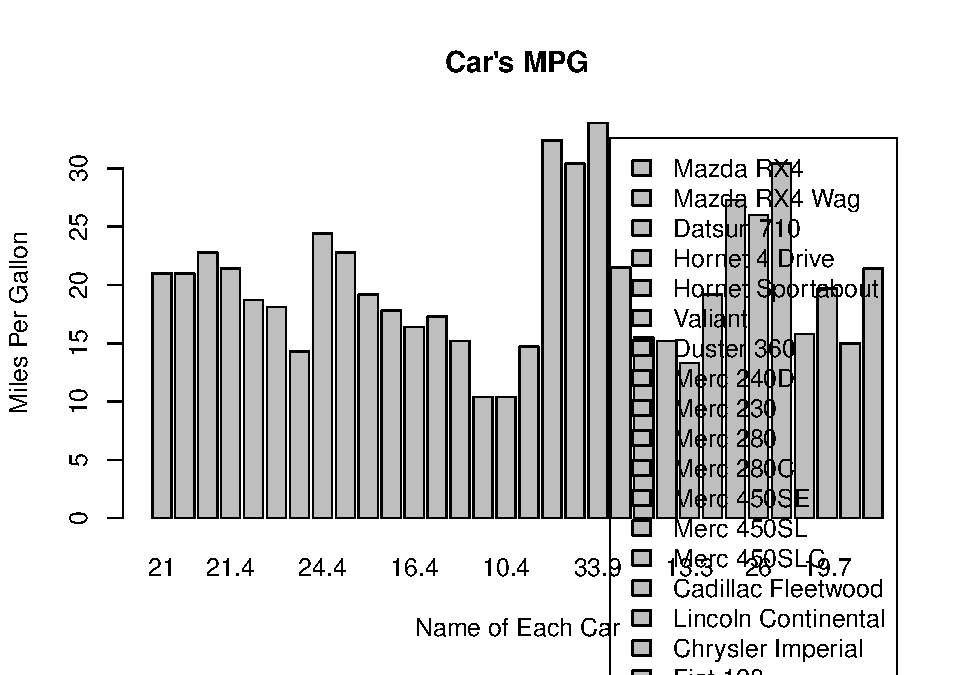
\includegraphics{CA2_DataAnalysis_files/figure-latex/unnamed-chunk-6-1.pdf}

\begin{enumerate}
\def\labelenumi{\arabic{enumi}.}
\setcounter{enumi}{1}
\tightlist
\item
  Now plot a scatterplot of \texttt{mpg} vs.~\texttt{hp}. Find the
  correlation coefficient between these two variables. Does it reflect
  what you see on the plot?
\end{enumerate}

\begin{Shaded}
\begin{Highlighting}[]
\KeywordTok{plot}\NormalTok{(}\DataTypeTok{x =}\NormalTok{ mtcars_dat}\OperatorTok{$}\NormalTok{mpg, }\DataTypeTok{y =}\NormalTok{ mtcars_dat}\OperatorTok{$}\NormalTok{hp, }\DataTypeTok{xlab =} \StringTok{"Miles/(US) gallon"}\NormalTok{, }\DataTypeTok{ylab =} \StringTok{"Gross Horsepower"}\NormalTok{, }\DataTypeTok{main =} \StringTok{"Gross horsepower vs Miles per Gallon"}\NormalTok{)}
\end{Highlighting}
\end{Shaded}

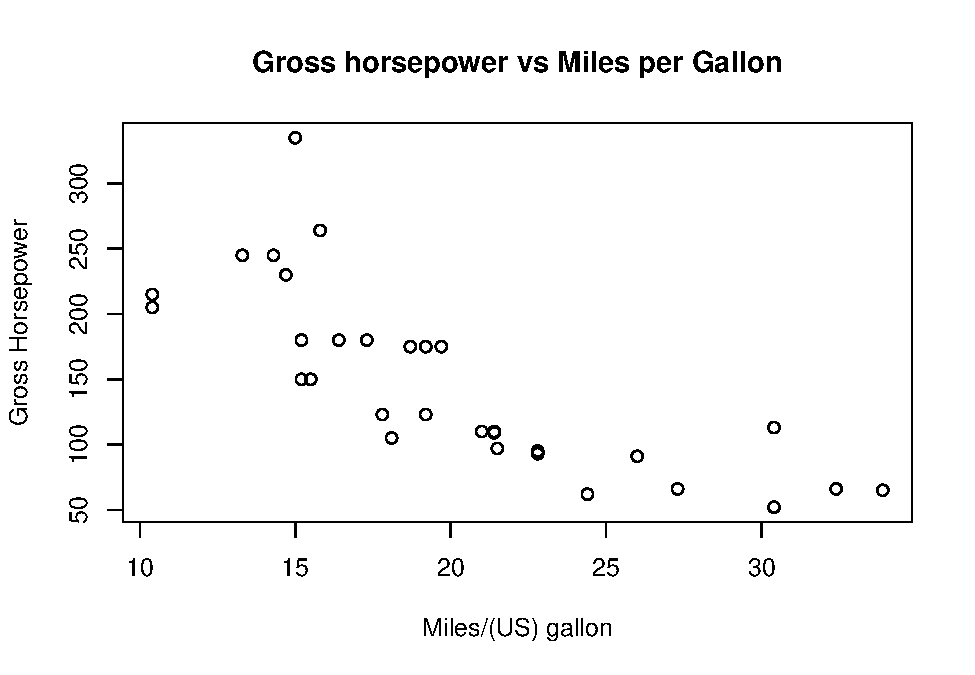
\includegraphics{CA2_DataAnalysis_files/figure-latex/unnamed-chunk-7-1.pdf}

\begin{Shaded}
\begin{Highlighting}[]
\KeywordTok{cor}\NormalTok{(mtcars_dat}\OperatorTok{$}\NormalTok{mpg,mtcars_dat}\OperatorTok{$}\NormalTok{hp)}
\end{Highlighting}
\end{Shaded}

\begin{verbatim}
## [1] -0.7761684
\end{verbatim}

\begin{verbatim}
The correlation coefficient between these two variables is r=-0.78, showing that they are generally negatively correlated, which can be seen on the plot as well. 
\end{verbatim}

\begin{enumerate}
\def\labelenumi{\arabic{enumi}.}
\setcounter{enumi}{2}
\tightlist
\item
  Plot a scatterplot of \texttt{drat} and \texttt{hp}. Do you observe
  any linear trend?
\end{enumerate}

\begin{Shaded}
\begin{Highlighting}[]
\KeywordTok{plot}\NormalTok{(}\DataTypeTok{x =}\NormalTok{ mtcars_dat}\OperatorTok{$}\NormalTok{drat, }\DataTypeTok{y =}\NormalTok{ mtcars_dat}\OperatorTok{$}\NormalTok{hp, }\DataTypeTok{xlab =} \StringTok{"Rear axle ratio"}\NormalTok{, }\DataTypeTok{ylab =} \StringTok{"Gross horsepower"}\NormalTok{, }\DataTypeTok{main =} \StringTok{"Gross horsepower vs Rear axle ratio"}\NormalTok{)}
\end{Highlighting}
\end{Shaded}

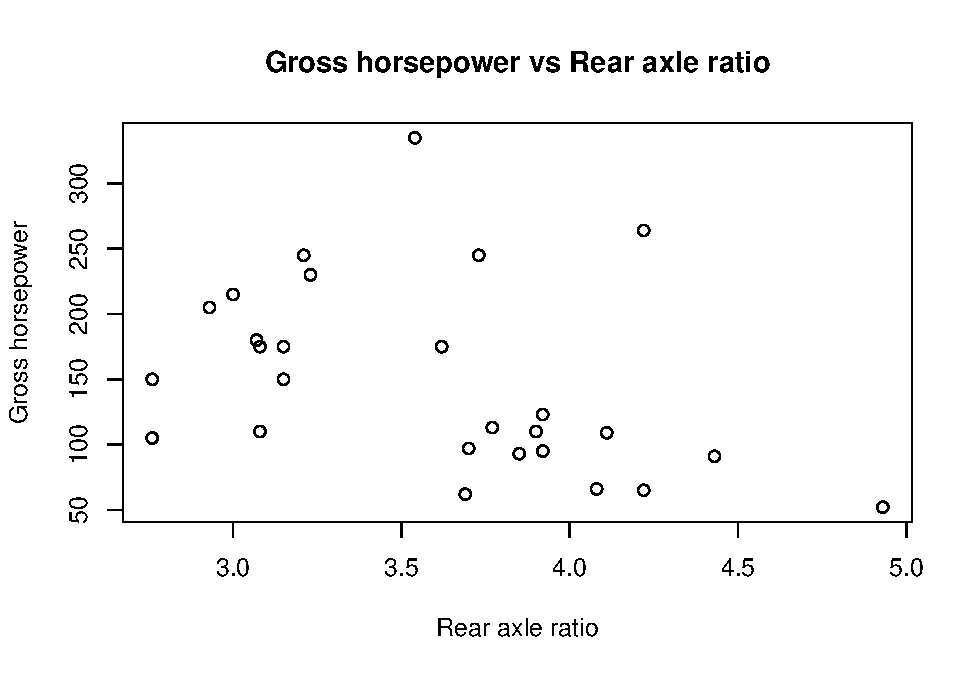
\includegraphics{CA2_DataAnalysis_files/figure-latex/unnamed-chunk-8-1.pdf}

\begin{Shaded}
\begin{Highlighting}[]
\KeywordTok{cor}\NormalTok{(mtcars_dat}\OperatorTok{$}\NormalTok{drat,mtcars_dat}\OperatorTok{$}\NormalTok{hp)}
\end{Highlighting}
\end{Shaded}

\begin{verbatim}
## [1] -0.4487591
\end{verbatim}

\begin{verbatim}
From the plot, there is no clear linear trend between the two variables. This result can be proved by the correlation calculation as well, where r=-0.45 showing that they have a loosely relation.
\end{verbatim}

\hypertarget{create-advanced-plots}{%
\subsubsection{Create advanced plots}\label{create-advanced-plots}}

If you are a JAVA programmer, then you might anticipate a plotting
toolbox to establish graphs layer-by-layer interactively. The
\texttt{ggplot2} package endows \textbf{R} with more advanced and
powerful visualization techniques like this. Explore more in
\href{https://cran.r-project.org/web/packages/ggplot2/ggplot2.pdf}{the
online package manual}.

\begin{Shaded}
\begin{Highlighting}[]
\NormalTok{mu <-}\StringTok{ }\KeywordTok{mean}\NormalTok{(iris}\OperatorTok{$}\NormalTok{Sepal.Length)}
\NormalTok{sigma <-}\StringTok{ }\KeywordTok{sd}\NormalTok{(iris}\OperatorTok{$}\NormalTok{Sepal.Length)}
\KeywordTok{ggplot}\NormalTok{(iris, }\KeywordTok{aes}\NormalTok{(Sepal.Length)) }\OperatorTok{+}
\StringTok{  }\KeywordTok{geom_histogram}\NormalTok{( }\KeywordTok{aes}\NormalTok{(}\DataTypeTok{y =}\NormalTok{ ..density..),}
                  \DataTypeTok{bins =} \DecValTok{8}\NormalTok{, }\DataTypeTok{color =} \StringTok{"black"}\NormalTok{, }\DataTypeTok{fill =} \StringTok{"white"}\NormalTok{) }\OperatorTok{+}
\StringTok{  }\KeywordTok{geom_density}\NormalTok{(}\KeywordTok{aes}\NormalTok{(}\DataTypeTok{color =} \StringTok{"blue"}\NormalTok{)) }\OperatorTok{+}
\StringTok{  }\KeywordTok{stat_function}\NormalTok{( }\KeywordTok{aes}\NormalTok{(}\DataTypeTok{color =} \StringTok{"red"}\NormalTok{), }
                 \DataTypeTok{fun =}\NormalTok{ dnorm, }\DataTypeTok{args =} \KeywordTok{list}\NormalTok{(}\DataTypeTok{mean =}\NormalTok{ mu, }\DataTypeTok{sd =}\NormalTok{ sigma)) }\OperatorTok{+}
\StringTok{  }\KeywordTok{labs}\NormalTok{(}\DataTypeTok{title =} \StringTok{"Histogram of Sepal_Length"}\NormalTok{) }\OperatorTok{+}
\StringTok{  }\KeywordTok{scale_color_identity}\NormalTok{( }\DataTypeTok{name   =} \StringTok{"Density Estimate"}\NormalTok{,}
                        \DataTypeTok{guide  =} \StringTok{"legend"}\NormalTok{,}
                        \DataTypeTok{labels =} \KeywordTok{c}\NormalTok{(}\StringTok{"Kernel"}\NormalTok{, }\StringTok{"Normal"}\NormalTok{)) }\OperatorTok{+}
\StringTok{  }\KeywordTok{theme_bw}\NormalTok{()}
\end{Highlighting}
\end{Shaded}

\hypertarget{further-analysis-and-practice}{%
\subsubsection{Further Analysis and
Practice}\label{further-analysis-and-practice}}

Let's again load the \texttt{mtcars} dataset into R. Again, this dataset
is actually available in base R, but to practice the input/output
features in R we'll load it from a CSV (Comma Separated File). Make sure
the file ``mtcars.csv'' is in the same directory as this Markdown file,
set the working directory, and run the following command.

\begin{Shaded}
\begin{Highlighting}[]
\CommentTok{# We will first read in the data using the read.table() command,}
\NormalTok{my.dat =}\StringTok{ }\KeywordTok{read.table}\NormalTok{(}\StringTok{"mtcars.csv"}\NormalTok{, }\DataTypeTok{sep =} \StringTok{","}\NormalTok{, }\DataTypeTok{header =} \OtherTok{TRUE}\NormalTok{)}
\CommentTok{# then do just a bit of cleaning up:}
\KeywordTok{row.names}\NormalTok{(my.dat) =}\StringTok{ }\NormalTok{my.dat}\OperatorTok{$}\NormalTok{X}
\NormalTok{my.dat =}\StringTok{ }\NormalTok{my.dat[,}\OperatorTok{-}\DecValTok{1}\NormalTok{]}
\CommentTok{# It may have been easier here to use the read.csv() function.  Check out it's manual page ?read.csv()}
\CommentTok{# to figure out why.}
\end{Highlighting}
\end{Shaded}

The \emph{read.table()} function can be used to import, or read, data
from pre-saved files including .txt, .csv, .xlsx or files available
online. Similarly, the \emph{write.table()} function can be used to
write a saved \textbf{R} variable to a .txt, .csv, or .xlsx file.

\hypertarget{questions-2}{%
\subsubsection{Questions}\label{questions-2}}

\begin{enumerate}
\def\labelenumi{\arabic{enumi}.}
\tightlist
\item
  Remember that once we read in a dataset with \textbf{R}, the value
  will be a data.frame type. Try to change our data.frame into a matrix
  type by using, for example, the \emph{dat.1 = as.matrix(dat.1)}
  command.
\end{enumerate}

\begin{Shaded}
\begin{Highlighting}[]
\NormalTok{my.dat =}\StringTok{ }\KeywordTok{as.matrix}\NormalTok{(my.dat)}
\end{Highlighting}
\end{Shaded}

\begin{enumerate}
\def\labelenumi{\arabic{enumi}.}
\setcounter{enumi}{1}
\tightlist
\item
  Calculate the standard deviation and the 5-number summary for each of
  the columns using the \emph{summary()} and \emph{sd()}. Also, estimate
  the coefficient of variation (\(c_v = \sigma / \mu\)) for each of the
  columns of our dataset.
\end{enumerate}

\begin{Shaded}
\begin{Highlighting}[]
\CommentTok{#Standard deviation of each column}
\ControlFlowTok{for}\NormalTok{ (i }\ControlFlowTok{in} \DecValTok{1}\OperatorTok{:}\KeywordTok{ncol}\NormalTok{(my.dat)) \{}
  \KeywordTok{print}\NormalTok{(}\KeywordTok{paste}\NormalTok{(}\StringTok{"The standard deviation of "}\NormalTok{,i,}\StringTok{" column is "}\NormalTok{,}\KeywordTok{sd}\NormalTok{(my.dat[,i])))}
\NormalTok{\}}
\end{Highlighting}
\end{Shaded}

\begin{verbatim}
## [1] "The standard deviation of  1  column is  6.0269480520891"
## [1] "The standard deviation of  2  column is  1.78592164694654"
## [1] "The standard deviation of  3  column is  123.938693831382"
## [1] "The standard deviation of  4  column is  68.5628684893206"
## [1] "The standard deviation of  5  column is  0.534678736070971"
## [1] "The standard deviation of  6  column is  0.978457442989697"
## [1] "The standard deviation of  7  column is  1.78694323609684"
## [1] "The standard deviation of  8  column is  0.504016128774185"
## [1] "The standard deviation of  9  column is  0.498990917235846"
## [1] "The standard deviation of  10  column is  0.737804065256947"
## [1] "The standard deviation of  11  column is  1.61519997763185"
\end{verbatim}

\begin{Shaded}
\begin{Highlighting}[]
\CommentTok{#5-number Summary for each column}
\KeywordTok{summary}\NormalTok{(my.dat)}
\end{Highlighting}
\end{Shaded}

\begin{verbatim}
##       mpg             cyl             disp             hp       
##  Min.   :10.40   Min.   :4.000   Min.   : 71.1   Min.   : 52.0  
##  1st Qu.:15.43   1st Qu.:4.000   1st Qu.:120.8   1st Qu.: 96.5  
##  Median :19.20   Median :6.000   Median :196.3   Median :123.0  
##  Mean   :20.09   Mean   :6.188   Mean   :230.7   Mean   :146.7  
##  3rd Qu.:22.80   3rd Qu.:8.000   3rd Qu.:326.0   3rd Qu.:180.0  
##  Max.   :33.90   Max.   :8.000   Max.   :472.0   Max.   :335.0  
##       drat             wt             qsec             vs        
##  Min.   :2.760   Min.   :1.513   Min.   :14.50   Min.   :0.0000  
##  1st Qu.:3.080   1st Qu.:2.581   1st Qu.:16.89   1st Qu.:0.0000  
##  Median :3.695   Median :3.325   Median :17.71   Median :0.0000  
##  Mean   :3.597   Mean   :3.217   Mean   :17.85   Mean   :0.4375  
##  3rd Qu.:3.920   3rd Qu.:3.610   3rd Qu.:18.90   3rd Qu.:1.0000  
##  Max.   :4.930   Max.   :5.424   Max.   :22.90   Max.   :1.0000  
##        am              gear            carb      
##  Min.   :0.0000   Min.   :3.000   Min.   :1.000  
##  1st Qu.:0.0000   1st Qu.:3.000   1st Qu.:2.000  
##  Median :0.0000   Median :4.000   Median :2.000  
##  Mean   :0.4062   Mean   :3.688   Mean   :2.812  
##  3rd Qu.:1.0000   3rd Qu.:4.000   3rd Qu.:4.000  
##  Max.   :1.0000   Max.   :5.000   Max.   :8.000
\end{verbatim}

\begin{verbatim}
The estimation of the coefficient of variance are 0.3, 0.3, 0.5, 0.5, 0.15, 0.3, 0.1, 1.2, 1.2, 0.2, 0.6.
\end{verbatim}

\begin{enumerate}
\def\labelenumi{\arabic{enumi}.}
\setcounter{enumi}{2}
\tightlist
\item
  For columns 1, 3, and 6, find the following information:
\end{enumerate}

\begin{itemize}
\tightlist
\item
  Whether the data is integer or non-integer valued
\item
  Mean
\item
  Median
\item
  Standard deviation
\item
  Coefficient of variation (if applicable) (Use the \emph{summary()} and
  \emph{sd()} commands.)
\end{itemize}

\begin{Shaded}
\begin{Highlighting}[]
\ControlFlowTok{for}\NormalTok{ (i }\ControlFlowTok{in} \KeywordTok{c}\NormalTok{(}\DecValTok{1}\NormalTok{,}\DecValTok{3}\NormalTok{,}\DecValTok{6}\NormalTok{)) \{}
  \KeywordTok{print}\NormalTok{(}\KeywordTok{paste}\NormalTok{(}\StringTok{"For column "}\NormalTok{,i,}\StringTok{": "}\NormalTok{))}
  \KeywordTok{print}\NormalTok{(}\KeywordTok{paste}\NormalTok{(}\StringTok{"Mean: "}\NormalTok{,}\KeywordTok{as.numeric}\NormalTok{(}\KeywordTok{summary}\NormalTok{(my.dat[,i])[}\DecValTok{4}\NormalTok{])))}
  \KeywordTok{print}\NormalTok{(}\KeywordTok{paste}\NormalTok{(}\StringTok{"Median: "}\NormalTok{,}\KeywordTok{as.numeric}\NormalTok{(}\KeywordTok{summary}\NormalTok{(my.dat[,i])[}\DecValTok{3}\NormalTok{])))}
  \KeywordTok{print}\NormalTok{(}\KeywordTok{paste}\NormalTok{(}\StringTok{"Standard deviation: "}\NormalTok{,}\KeywordTok{sd}\NormalTok{(my.dat[,i])))}
  \KeywordTok{print}\NormalTok{(}\KeywordTok{paste}\NormalTok{(}\StringTok{"Coefficient of variation: "}\NormalTok{,}\KeywordTok{sd}\NormalTok{(my.dat[,i])}\OperatorTok{/}\KeywordTok{as.numeric}\NormalTok{(}\KeywordTok{summary}\NormalTok{(my.dat[,i])[}\DecValTok{4}\NormalTok{])))}
\NormalTok{\}}
\end{Highlighting}
\end{Shaded}

\begin{verbatim}
## [1] "For column  1 : "
## [1] "Mean:  20.090625"
## [1] "Median:  19.2"
## [1] "Standard deviation:  6.0269480520891"
## [1] "Coefficient of variation:  0.299988081609661"
## [1] "For column  3 : "
## [1] "Mean:  230.721875"
## [1] "Median:  196.3"
## [1] "Standard deviation:  123.938693831382"
## [1] "Coefficient of variation:  0.537177906652249"
## [1] "For column  6 : "
## [1] "Mean:  3.21725"
## [1] "Median:  3.325"
## [1] "Standard deviation:  0.978457442989697"
## [1] "Coefficient of variation:  0.304128508194793"
\end{verbatim}

\begin{enumerate}
\def\labelenumi{\arabic{enumi}.}
\setcounter{enumi}{3}
\tightlist
\item
  Comment on the similarities and differences between each of these
  samples.
\end{enumerate}

\begin{verbatim}
Three columns have very different mean and median value: column 1 has the largest values, column 3 the second, and the column 6 the last.

However, their mean and median are very closed, and they have similar coefficient of variance: column 1 is 0.3, column 3 is 0.5, and column 6 is 0.3.
\end{verbatim}

\hypertarget{empirical-cumulative-distribution-functions}{%
\subsection{Empirical cumulative distribution
functions}\label{empirical-cumulative-distribution-functions}}

The empirical cumulative distribution function (ECDF) of a random sample
provides a summary of the sample based on the order (smallest to
largest) of the sample. When the sample is perceived to come from a
probability distribution, the ECDF can be used to estimate the true
cumulative distribution function of the sample. We can calculate the
ECDF of a sample by using the \emph{ecdf()} command in \textbf{R}. Plot
the ECDF of the first, fourth, and fifth columns.

\begin{Shaded}
\begin{Highlighting}[]
\CommentTok{# plot the ecdf of car miles per gallon and color it green}
\KeywordTok{plot}\NormalTok{(}\KeywordTok{ecdf}\NormalTok{(my.dat[,}\DecValTok{1}\NormalTok{]), }\DataTypeTok{col =} \StringTok{"green"}\NormalTok{)}
\end{Highlighting}
\end{Shaded}

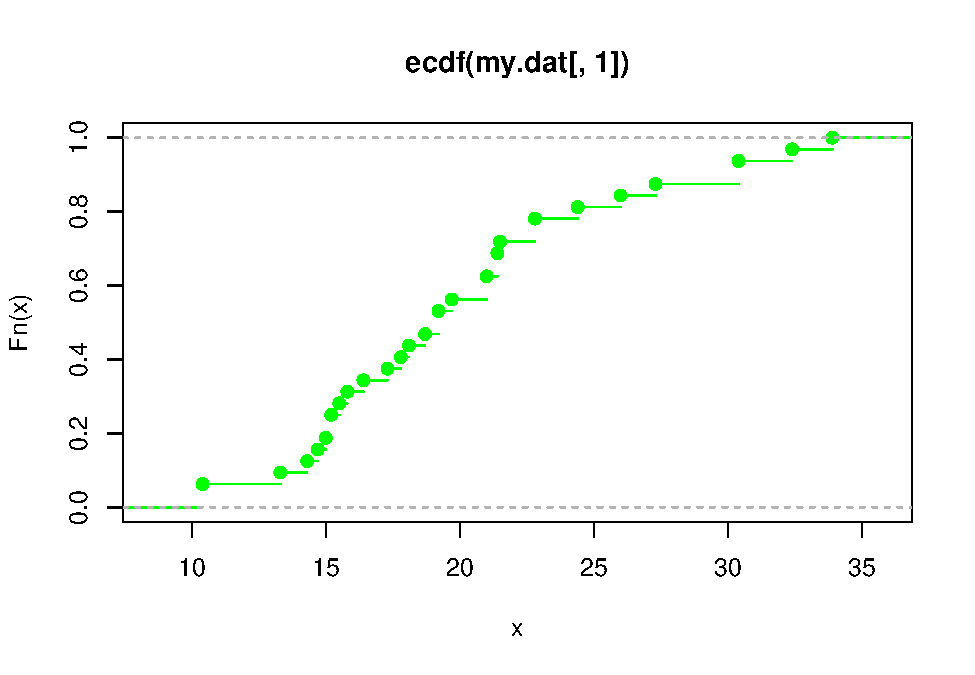
\includegraphics{CA2_DataAnalysis_files/figure-latex/unnamed-chunk-14-1.pdf}

\begin{Shaded}
\begin{Highlighting}[]
\CommentTok{# plot the ecdf of rear axle ratio, color it blue}
\KeywordTok{plot}\NormalTok{(}\KeywordTok{ecdf}\NormalTok{(my.dat[,}\DecValTok{4}\NormalTok{]), }\DataTypeTok{col =} \StringTok{"blue"}\NormalTok{)}
\end{Highlighting}
\end{Shaded}

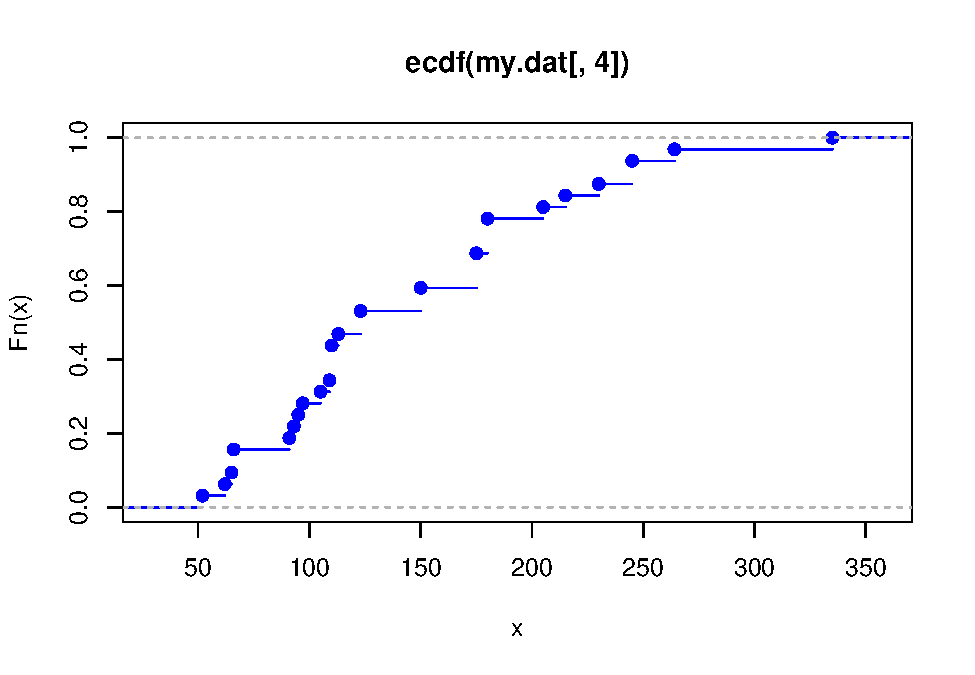
\includegraphics{CA2_DataAnalysis_files/figure-latex/unnamed-chunk-14-2.pdf}

\begin{Shaded}
\begin{Highlighting}[]
\CommentTok{# plot the ecdf of car weight, color it red}
\KeywordTok{plot}\NormalTok{(}\KeywordTok{ecdf}\NormalTok{(my.dat[,}\DecValTok{5}\NormalTok{]), }\DataTypeTok{col =} \StringTok{"red"}\NormalTok{)}
\end{Highlighting}
\end{Shaded}

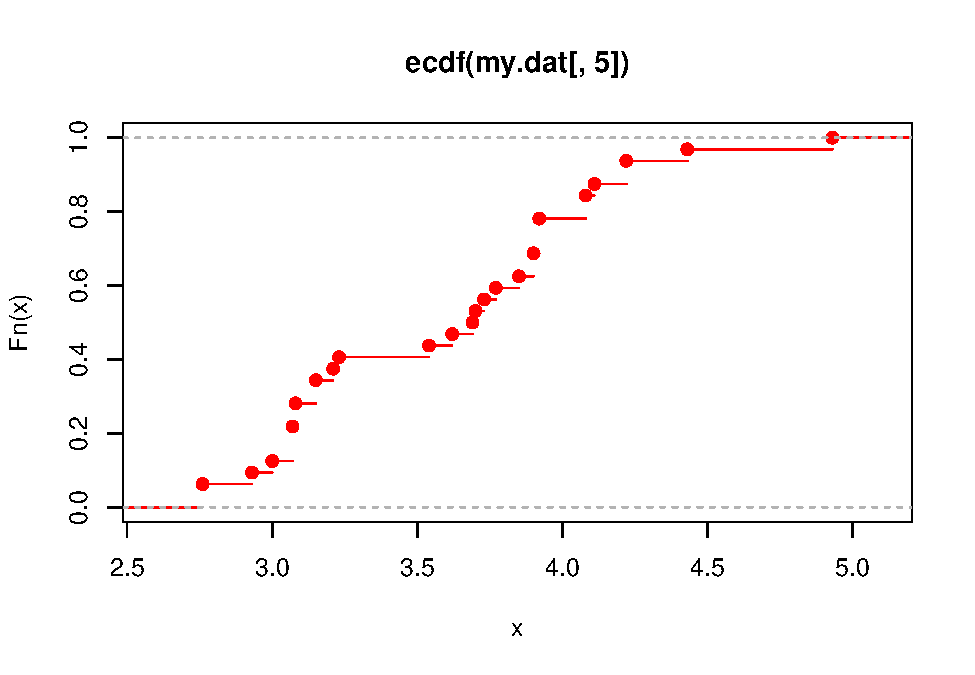
\includegraphics{CA2_DataAnalysis_files/figure-latex/unnamed-chunk-14-3.pdf}

Next, plot the histograms of each of the same columns using the
following code:

\begin{Shaded}
\begin{Highlighting}[]
\CommentTok{# plot the histogram of x1}
\KeywordTok{hist}\NormalTok{(my.dat[,}\DecValTok{1}\NormalTok{], }\DataTypeTok{main =} \StringTok{"Histogram of Miles per Gallon"}\NormalTok{)}
\end{Highlighting}
\end{Shaded}

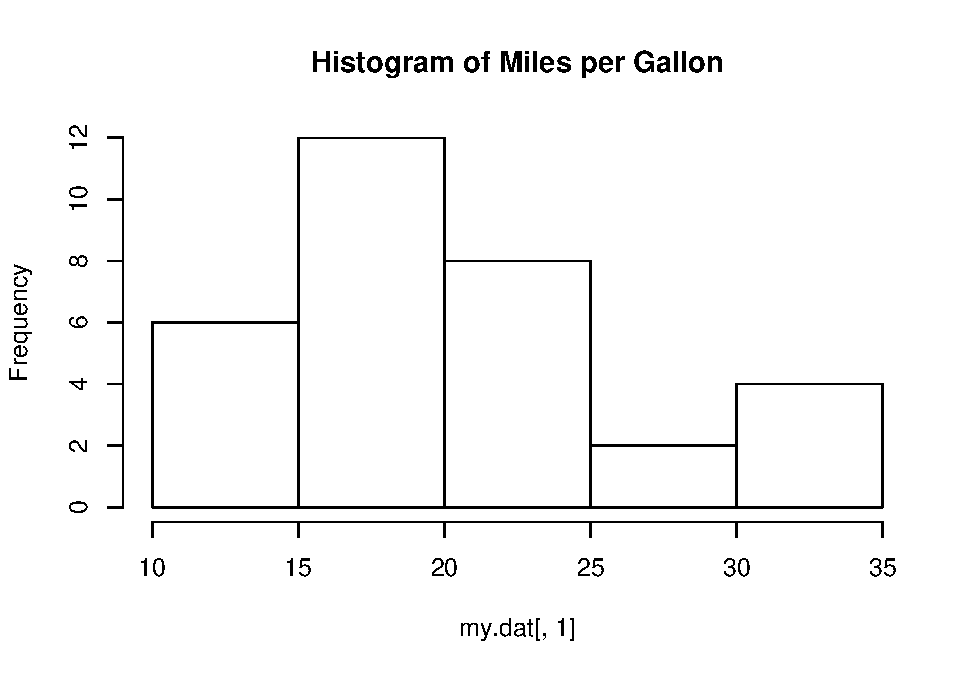
\includegraphics{CA2_DataAnalysis_files/figure-latex/unnamed-chunk-15-1.pdf}

\begin{Shaded}
\begin{Highlighting}[]
\KeywordTok{hist}\NormalTok{(my.dat[,}\DecValTok{4}\NormalTok{], }\DataTypeTok{main =} \StringTok{"Histogram of Rear Axle Ratio"}\NormalTok{)}
\end{Highlighting}
\end{Shaded}

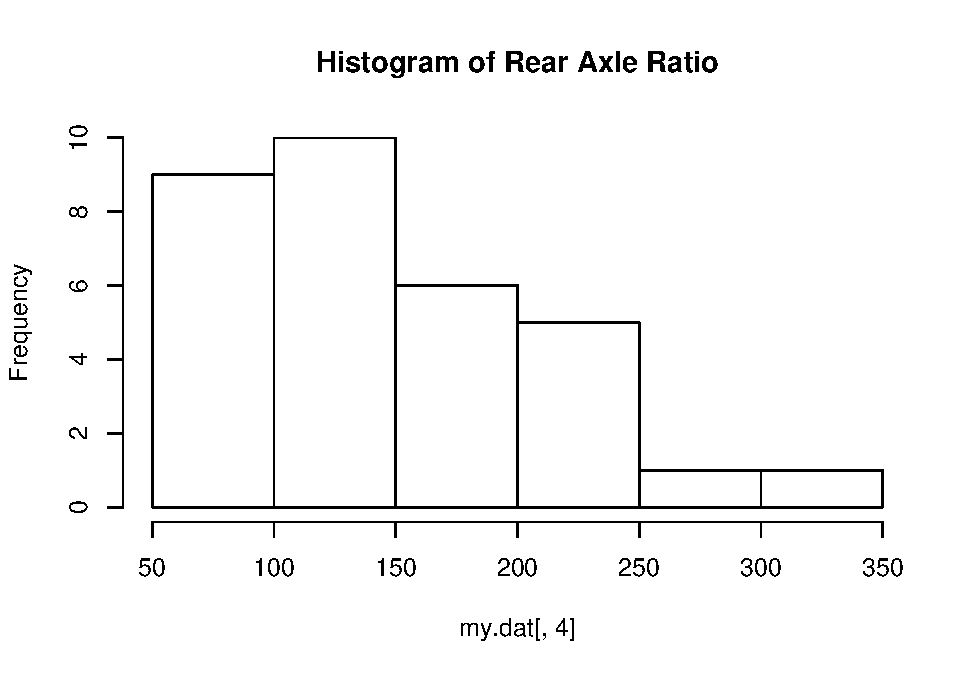
\includegraphics{CA2_DataAnalysis_files/figure-latex/unnamed-chunk-15-2.pdf}

\begin{Shaded}
\begin{Highlighting}[]
\KeywordTok{hist}\NormalTok{(my.dat[,}\DecValTok{5}\NormalTok{], }\DataTypeTok{main =} \StringTok{"Histogram of Car Weight"}\NormalTok{)}
\end{Highlighting}
\end{Shaded}

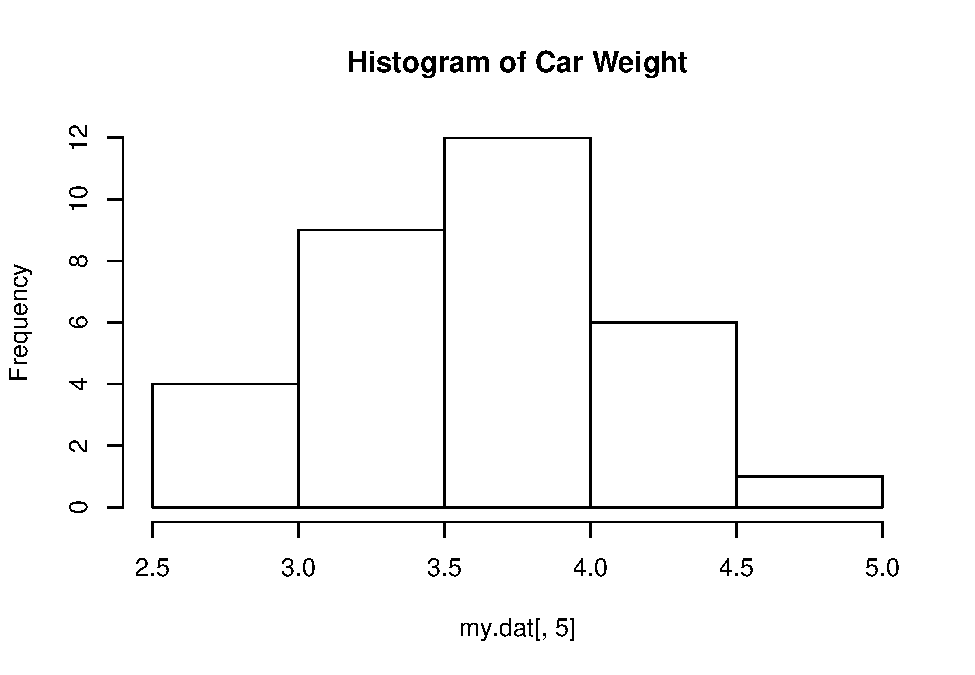
\includegraphics{CA2_DataAnalysis_files/figure-latex/unnamed-chunk-15-3.pdf}
\#\#\# Questions

\begin{enumerate}
\def\labelenumi{\arabic{enumi}.}
\tightlist
\item
  Note that the means of \texttt{drat} and \texttt{wt} are approximately
  equal. It may be tempting to think that two samples are similar (or
  even that they are samples from the same population) when they share
  the same mean. Do the ECDFs of these variables support this claim?
  Examine closely the beginning of each ECDF.
\end{enumerate}

YOUR ANSWER HERE.

\begin{enumerate}
\def\labelenumi{\arabic{enumi}.}
\setcounter{enumi}{1}
\tightlist
\item
  Comment on what the histograms of each of these samples provides. Do
  these histograms support the claim that the samples are realizations
  of the same random variable?
\end{enumerate}

YOUR COMMENT HERE.

\hypertarget{bivariate-relationships-and-correlation}{%
\subsection{Bivariate relationships and
Correlation}\label{bivariate-relationships-and-correlation}}

Correlation and covariance are two descriptive statistics that quantify
the association between two variables. In \textbf{R}, we can calculate
the sample correlation between two quantitative variables \(x\) and
\(y\) using the \emph{cor(x,y)} command. Similarly, we can use the
\emph{cov(x,y)} command to calculate the covariance between \(x\) and
\(y\). Calculate the pairwise correlations and covariances between
\texttt{hp}, \texttt{drat}, and \texttt{weight} using the code below:

\begin{Shaded}
\begin{Highlighting}[]
\CommentTok{# calculate pairwise covariances}
\KeywordTok{attach}\NormalTok{(my.dat)}
\NormalTok{cov}\FloatTok{.45}\NormalTok{ =}\StringTok{ }\KeywordTok{cov}\NormalTok{(hp,drat)}
\NormalTok{cov}\FloatTok{.46}\NormalTok{ =}\StringTok{ }\KeywordTok{cov}\NormalTok{(hp,wt)}
\NormalTok{cov}\FloatTok{.56}\NormalTok{ =}\StringTok{ }\KeywordTok{cov}\NormalTok{(drat,wt)}

\CommentTok{# calculate pairwise correlations}
\NormalTok{cor}\FloatTok{.45}\NormalTok{ =}\StringTok{ }\KeywordTok{cor}\NormalTok{(hp,drat)}
\NormalTok{cor}\FloatTok{.46}\NormalTok{ =}\StringTok{ }\KeywordTok{cor}\NormalTok{(hp,wt)}
\NormalTok{cor}\FloatTok{.56}\NormalTok{ =}\StringTok{ }\KeywordTok{cor}\NormalTok{(drat,wt)}
\KeywordTok{detach}\NormalTok{(my.dat)}
\end{Highlighting}
\end{Shaded}

Using the \emph{plot()} command, plot a scatterplot between each pair of
the above three variables. Be sure to appropriately label each of these
plots.

\begin{Shaded}
\begin{Highlighting}[]
\NormalTok{YOUR CODE HERE}
\end{Highlighting}
\end{Shaded}

\hypertarget{questions-3}{%
\subsubsection{Questions}\label{questions-3}}

\begin{enumerate}
\def\labelenumi{\arabic{enumi}.}
\tightlist
\item
  Verify that for each of the pairs (\texttt{hp}, \texttt{drat}),
  (\texttt{hp}, \texttt{wt}), and (\texttt{drat}, \texttt{wt}), the
  correlation is the quotient of the covariance and the product of the
  standard deviations.
\end{enumerate}

\begin{Shaded}
\begin{Highlighting}[]
\NormalTok{YOUR CODE HERE}
\end{Highlighting}
\end{Shaded}

\begin{enumerate}
\def\labelenumi{\arabic{enumi}.}
\setcounter{enumi}{1}
\tightlist
\item
  Comment on each of the generated scatterplots. What does the
  correlation tell us about the relationships shown in the scatterplots?
  Does the covariance provide similar information as the correlation?
\end{enumerate}

YOUR COMMENT HERE.

\hypertarget{t-tests}{%
\subsection{t-tests}\label{t-tests}}

One way to test for statistically significant differences between two
samples is to use a formal hypothesis test known as the t-test. There
are two types of t-statistics that we will consider: the
\emph{Student's} t-statistic and the \emph{Welsh} t-statistic. These
statistics are used in different situations depending on the variance of
the two samples being compared. You can use the typical Student's t-test
whenever variances are the same, but should use Welsh's whenever the
variances are not equal.

Consider comparing two samples \(x\) and \(y\). We can calculate either
of these t-test statistics using the function \emph{t.test()}. In
particular, if the variance of the two samples are \textbf{not} equal,
then we use the command \emph{t.test(x, y, var.equal = FALSE)}. If the
variances \textbf{are} equal, then we use the command \emph{t.test(x, y,
var.equal = TRUE)}.

\hypertarget{questions-4}{%
\subsubsection{Questions}\label{questions-4}}

\begin{enumerate}
\def\labelenumi{\arabic{enumi}.}
\tightlist
\item
  Which t-statistic is appropriate to compare the samples \texttt{hp}
  and \texttt{wt}? How about \texttt{drat} and \texttt{vs}?
\end{enumerate}

YOU ANSWERS HERE.

\begin{enumerate}
\def\labelenumi{\arabic{enumi}.}
\setcounter{enumi}{1}
\tightlist
\item
  Calculate the t-statistic to compare \texttt{hp} and \texttt{wt}. Are
  the two samples statistically significantly different at a 0.05 level?
\end{enumerate}

\begin{Shaded}
\begin{Highlighting}[]
\NormalTok{YOUR CODE, AND RESPONSE, HERE}
\end{Highlighting}
\end{Shaded}

\begin{enumerate}
\def\labelenumi{\arabic{enumi}.}
\setcounter{enumi}{2}
\tightlist
\item
  Repeat (2) for \texttt{drat} and \texttt{vs}.
\end{enumerate}

\begin{Shaded}
\begin{Highlighting}[]
\NormalTok{YOUR CODE, AND RESPONSE, HERE}
\end{Highlighting}
\end{Shaded}

\hypertarget{fishers-iris-data}{%
\subsection{Fisher's iris data}\label{fishers-iris-data}}

Now we will apply the above techniques to further explore the
\emph{iris} data set in \textbf{R}. Suppose we want to study the data in
the \emph{iris} dataset by flower species. It is easy in \textbf{R} to
subset datasets based on there variables. For example:

\begin{Shaded}
\begin{Highlighting}[]
\CommentTok{# Load the iris data}
\KeywordTok{data}\NormalTok{(iris)}

\CommentTok{# Make the setosa species subset}
\NormalTok{iris.setosa =}\StringTok{ }\NormalTok{iris[iris}\OperatorTok{$}\NormalTok{Species }\OperatorTok{==}\StringTok{ "setosa"}\NormalTok{, ]}

\CommentTok{# Look at the five-number summary for only the setosa species}
\KeywordTok{summary}\NormalTok{(iris.setosa)}
\end{Highlighting}
\end{Shaded}

As you work with more datasets/subsets and more variables, it can become
repetitive to call variables via \$. A useful function in \textbf{R} is
\emph{with()}, which wraps around your code and specifies which dataset
to work with. Try the following examples:

\begin{Shaded}
\begin{Highlighting}[]
\CommentTok{#Plot a scatterplot between the sepal length and the petal length}
\KeywordTok{with}\NormalTok{(iris, }
\KeywordTok{plot}\NormalTok{(Sepal.Length, Petal.Length, }\DataTypeTok{xlab =} \StringTok{"Sepal Length"}\NormalTok{, }\DataTypeTok{ylab =} \StringTok{"Petal Length"}\NormalTok{))}

\CommentTok{#Plot a scatterplot between the sepal length and the petal length for only setosa species}
\KeywordTok{with}\NormalTok{(iris.setosa, }
\KeywordTok{plot}\NormalTok{(Sepal.Length, Petal.Length, }\DataTypeTok{xlab =} \StringTok{"Sepal Length"}\NormalTok{, }\DataTypeTok{ylab =} \StringTok{"Petal Length"}\NormalTok{))}
\end{Highlighting}
\end{Shaded}

Answer each of the following questions.

\hypertarget{questions-5}{%
\subsubsection{Questions}\label{questions-5}}

\begin{enumerate}
\def\labelenumi{\arabic{enumi}.}
\tightlist
\item
  Make a table that includes the five-number summary as well as standard
  deviation of the petal length and petal width of a) all 150 flowers,
  b) setosa species, and c) virginica species.
\end{enumerate}

\begin{Shaded}
\begin{Highlighting}[]
\NormalTok{YOUR CODE HERE}
\end{Highlighting}
\end{Shaded}

\begin{enumerate}
\def\labelenumi{\arabic{enumi}.}
\setcounter{enumi}{1}
\tightlist
\item
  Generate an appropriately labeled scatterplot showing the relationship
  between the petal length and petal width of all 150 flowers. Calculate
  the correlation and covariance between these two variables. Based on
  what you see, comment on the relationship between these two variables.
\end{enumerate}

\begin{Shaded}
\begin{Highlighting}[]
\NormalTok{YOUR CODE, AND COMMENT, HERE}
\end{Highlighting}
\end{Shaded}

\begin{enumerate}
\def\labelenumi{\arabic{enumi}.}
\setcounter{enumi}{2}
\tightlist
\item
  Repeat part (b) for the petal length and petal width of a) just the
  \emph{setosa} species, and b) just the \emph{virginica} species.
  Comment on what the differences between these two scatterplots and any
  observations that may be useful in distinguishing the two species.
\end{enumerate}

\begin{Shaded}
\begin{Highlighting}[]
\NormalTok{YOUR CODE, AND COMMENTS, HERE}
\end{Highlighting}
\end{Shaded}

\begin{enumerate}
\def\labelenumi{\arabic{enumi}.}
\setcounter{enumi}{3}
\tightlist
\item
  Plot the ECDF of the petal length of the \emph{setosa} and the petal
  length of the \emph{virginica} species in two different plots. Do the
  same for the petal width of these two species. Be sure to
  appropriately label each of the four plots. What do these plots reveal
  about the relationship between these two species?
\end{enumerate}

\begin{Shaded}
\begin{Highlighting}[]
\NormalTok{YOUR CODE HERE}
\end{Highlighting}
\end{Shaded}

\begin{enumerate}
\def\labelenumi{\arabic{enumi}.}
\setcounter{enumi}{4}
\tightlist
\item
  Which t-statistic is appropriate for testing the difference between
  the petal length of the \emph{setosa} and \emph{virginica} species?
  Why? Calculate the t-statistic. Are the petal lengths between these
  two species statistically different?
\end{enumerate}

\begin{Shaded}
\begin{Highlighting}[]
\NormalTok{YOUR CODE, AND COMMENTS, HERE}
\end{Highlighting}
\end{Shaded}

\begin{enumerate}
\def\labelenumi{\arabic{enumi}.}
\setcounter{enumi}{5}
\tightlist
\item
  Which t-statistic is appropriate for testing the difference between
  the petal width of the \emph{setosa} and \emph{virginica} species?
  Why? Calculate the t-statistic. Are the petal widths between these two
  species statistically different?
\end{enumerate}

\begin{Shaded}
\begin{Highlighting}[]
\NormalTok{YOUR CODE, AND COMMENTS, HERE}
\end{Highlighting}
\end{Shaded}

\end{document}
